\documentclass[11pt,a4paper]{article}
\usepackage[margin=2.5cm]{geometry}
\usepackage[T1]{fontenc}
\usepackage[utf8]{inputenc}
\usepackage{lmodern,microtype,graphicx,booktabs,tabularx,longtable,array,caption,hyperref,float,pdflscape,xcolor}
\usepackage{enumitem}
\usepackage{dblfloatfix}
\graphicspath{{figures/}}
\setlength{\emergencystretch}{3em}
\sloppy
\setlength{\parindent}{0pt}\setlength{\parskip}{5pt}
\setlist{nosep,leftmargin=*}
\hypersetup{colorlinks=true,linkcolor=black,urlcolor=blue}
\newcommand{\var}[1]{\texttt{\detokenize{#1}}}

\title{\textbf{Dataset Report}\\Recognizing Albums from Any Packaging Image}
\author{
    TME 6015: AI/ML Workflow Design\\[6pt]
    Akinbobola Akin (3784664)
}
\date{November 5, 2026}

\begin{document}\maketitle

% ---------------------------------------------------------------
\section{Problem Statement}
Streaming platforms like Spotify, Apple Music and Deezer have made music easy to access. Each album on these platforms has one digital version, chosen as the official version of that album. But in practice, most popular albums exist in many physical versions. Artists, studios and labels release the same album again and again across countries, formats and anniversaries, with small changes to each release: a new sticker, a banner, a recoloured cover or even a completely different design. The return of vinyl has only added to this. US vinyl sales passed \$1 billion in 2025 for the first time since 1983~\cite{musicweek2026riaa}, and every new pressing is another edition to keep track of.

Music databases and marketplaces such as MusicBrainz~\cite{musicbrainz}, the Cover Art Archive~\cite{coverartarchive} and Discogs~\cite{discogs} have to catalogue all of these editions. The Cover Art Archive alone holds over 7.6 million images~\cite{caastats}, and volunteers tag each one by hand, often from a photo of just the disc or the back cover, which leads to mistakes.

This project treats the problem as image classification. Given a photo of any part of an album's packaging, the model predicts two things: which album it belongs to, out of ten, and which part of the packaging it shows: front, back, disc or booklet. A platform could use these predictions to suggest tags for new uploads and flag images whose tags look wrong, reducing manual work and catching errors before they spread.

% ---------------------------------------------------------------
\section{Dataset Description}
Appendix~\ref{app:terms} defines the music terms used in this report, such as album, release and packaging part.

The dataset has 2,223 images of album packaging from 10 albums, collected from the Cover Art Archive. Each image has two labels: the album it belongs to and the part of the packaging it shows, which is the front, back, disc or booklet. The images come from 899 different releases of these albums, and each release adds at most one image of each part. Most images are 500 pixels on the longest side.

\subsection{Data Collection}
To test whether a model can recognize an album across its editions, I needed albums that have been released many times. Older albums that fans treat as classics tend to get the most reissues, so I started with the Rolling Stone 500 Greatest Albums list~\cite{rollingstone500}. I removed live albums, compilations and Various Artists releases because they are not single studio albums, which left 467 candidates.

Next, I needed to know which of these albums had the most editions. I looked up each one on MusicBrainz, an open music database, and counted how many of its releases had a front cover on the Cover Art Archive, the image library linked to it. This count showed both how many editions an album had and how many images I could actually get. Of the 430 albums with a confirmed match, most had very few: the median was 17 releases with a front cover, and only 40 albums had 50 or more.

I took the 20 albums with the most releases, keeping only one album per artist, since two albums by the same artist could share a visual style and make the classes easier to confuse. I downloaded their front covers and chose the final 10 by looking through them myself. I wanted albums whose editions looked noticeably different from each other, and a mix of eras and genres. Because this step relied on my own judgement, I come back to it in the bias section.

I then kept only the four parts of the packaging that appear across most releases: front, back, disc and booklet. Images tagged as both back and spine were counted as backs, since the spine is just the edge of the back cover. I dropped rarer tags such as tray or obi because they had too few images to learn from. Some releases also had many images of the same part, like a booklet with 20 pages, so I kept one image per part per release to stop a single release from dominating the data.

\subsection{Number of Data Points}
Table~\ref{tab:counts} breaks the 2,223 images down by album and by part of the packaging. The releases column shows how many releases each album has on MusicBrainz, including those without artwork.

\begin{table}[H]\centering\small\caption{Images per album and packaging part}\label{tab:counts}
\begin{tabularx}{\linewidth}{@{}Xrrrrrr@{}}\toprule
Album & Releases & Front & Back & Disc & Booklet & Total\\\midrule
Paranoid (Black Sabbath) & 73 & 46 & 23 & 26 & 18 & 113\\
Darkness on the Edge of Town (Bruce Springsteen) & 167 & 145 & 128 & 140 & 29 & 442\\
Tapestry (Carole King) & 183 & 134 & 141 & 149 & 40 & 464\\
good kid, m.A.A.d city (Kendrick Lamar) & 73 & 57 & 33 & 30 & 14 & 134\\
Thriller (Michael Jackson) & 85 & 58 & 34 & 27 & 19 & 138\\
Kind of Blue (Miles Davis) & 137 & 104 & 85 & 82 & 31 & 302\\
Remain in Light (Talking Heads) & 94 & 69 & 56 & 68 & 22 & 215\\
Red (Taylor Swift) & 97 & 71 & 51 & 22 & 14 & 158\\
Tommy (The Who) & 54 & 43 & 27 & 26 & 18 & 114\\
The Joshua Tree (U2) & 66 & 48 & 35 & 36 & 24 & 143\\\midrule
Total & \textbf{1,029} & \textbf{775} & \textbf{613} & \textbf{606} & \textbf{229} & \textbf{2,223}\\
\bottomrule\end{tabularx}\end{table}

The counts are uneven, and this reflects how often each album has been reissued. Tapestry and Darkness on the Edge of Town each have over 440 images, while Paranoid and Tommy have about 110, so the largest album has roughly four times as many images as the smallest. The parts of the packaging are uneven too. Fronts are the most common because nearly every release has one, while booklets are the rarest, with only 229 images in total and as few as 14 for some albums. This happens because booklets mostly come with CDs, and vinyl and digital releases usually have none.

\subsection{Is the Data Enough}\label{sec:enough}
The number that matters most is not the image count but the number of releases. Images from the same release share the same print, wear and scanning conditions, so 2,223 images are closer to 899 independent examples.

These numbers are small for training a deep network from scratch, but they are workable for transfer learning. A model pre-trained on ImageNet~\cite{deng2009imagenet} already knows general features such as edges, textures, shapes and printed text, and these features carry over well to new image tasks~\cite{yosinski2014transferable,kornblith2019better}.

To check this instead of assuming it, I ran a pilot before training the full model. I split the data by release into training, validation and test sets of 1,537, 337 and 349 images, with every image from a release kept in the same set. I passed each image through a ResNet-50 pre-trained on ImageNet without changing its weights, and trained a simple logistic regression on the features it produced. I repeated this with 25\%, 50\%, 75\% and 100\% of the training releases and measured macro F1 on the validation set. The test set was not used.

\begin{figure}[H]\centering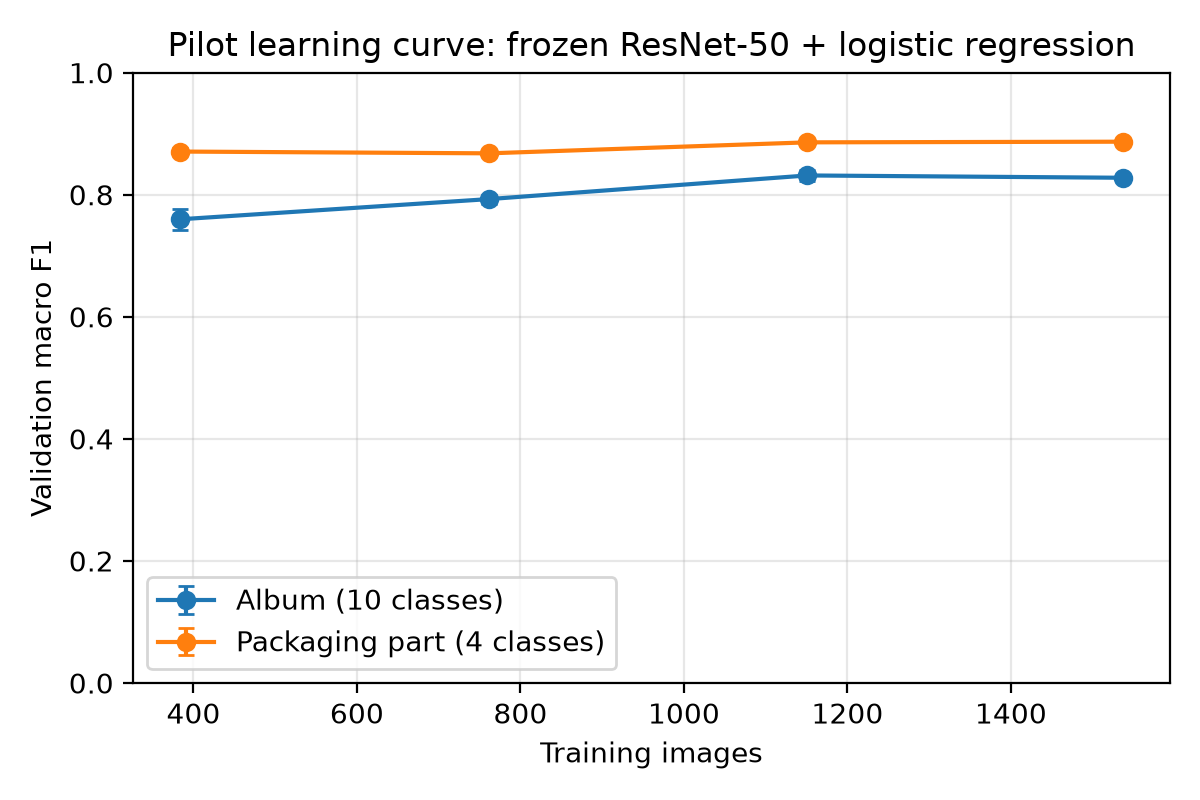
\includegraphics[width=0.75\linewidth]{pilot_learning_curve.png}\caption{Pilot learning curve: validation macro F1 against the number of training images for a frozen ResNet-50 with logistic regression. Error bars show the spread over three random subsets.}\label{fig:pilot}\end{figure}

Figure~\ref{fig:pilot} shows the results. For the album label, macro F1 rose from 0.76 with a quarter of the training data to 0.83 with three quarters, then stayed at 0.83 with all of it. For the packaging part, it started at 0.87 and only reached 0.89. Both curves flatten before the full training set, which suggests that more images of the same kind would add little, and that the dataset is large enough for transfer learning.

The pilot also shows where the model struggles. With all the training data, it named the right album for 96\% of fronts and 91\% of backs, but only 68\% of discs and 73\% of booklets. Since the overall curve has already flattened, these gaps more likely come from how hard discs and booklets are to recognize than from a lack of images. The booklet score also rests on only 33 validation images, so it is less certain. Fine-tuning the whole network in the final project, instead of keeping it frozen, should raise these scores, and I will study these two parts closely.

The test set has its own limit. It holds 349 images, but only 38 booklets in total and as few as 2 for some albums. A single mistake would move the score for those combinations a lot, so I will report results per album and per part separately, not for every album and part pair.

\subsection{Representativeness}
The model is meant to recognize the kind of album packaging images that people upload to music databases and marketplaces. For the dataset to represent that problem, it needs to cover the many forms an album takes across its editions, not just its best-known cover.

I did not hand-pick editions within an album. I included every release that had usable artwork, so the dataset follows the real spread of editions on the archive instead of my own idea of what an album should look like. The 899 releases in the dataset come from 56 countries. The largest groups are the United States (192), Europe-wide releases (138), Japan (79), Canada (76) and the United Kingdom (67). This matters because regional editions often change the packaging. Japanese releases, for example, often add an obi strip down the side of the cover.

The dataset also covers the main formats: 385 CD releases, 328 vinyl, 68 cassette and a few rarer ones such as 8-track and reel-to-reel. It also includes 100 digital releases, which add mostly front covers. Each format packages an album differently, with different sizes, materials and layouts, so the model sees the same album in many physical forms. The releases span every decade from the 1950s to the 2020s, which captures how reissues change over time, from original pressings to anniversary and deluxe editions.

The albums themselves cover a range of eras and genres. They go from Kind of Blue (1959) to Red and good kid, m.A.A.d city (2012), and include jazz, rock, heavy metal, singer-songwriter, new wave, pop and hip hop. Each album also has a different kind of variation. Some editions only add a sticker or banner, while others, like Thriller's anniversary editions and the two covers of good kid, m.A.A.d city, change the design completely.

Finally, the images come from many different uploaders. Some are clean scans and others are photos of worn copies with glare, stickers or price tags. This variety is close to what the model would face in real use.

The dataset does have limits. All 10 albums are well known, Western and mostly from before 1990, and scans outnumber phone photos. Booklets come mostly from CDs, with 181 of the 229 booklet images taken from CD releases.

\subsection{Steps to Ensure Enough Data}
I made several choices to get as many usable images as possible. The first was where I looked for albums. Critically acclaimed albums are the ones labels keep reissuing, so starting from the Rolling Stone 500 meant starting from albums likely to have many editions. Even then, most albums on the list had fewer than 20 releases with a front cover, which would never be enough. Ranking the list by edition count and keeping only the top albums meant I only worked with albums that had plenty of material.

When choosing tags, I looked for images I could keep without hurting the labels. Many back covers were tagged as both back and spine because the scan included the spine edge. These are still back covers, so I counted them as backs, which added 157 images to the back class.

During training, I will use data augmentation to give the model more variety from the images I have. Each time the model sees a training image, it gets a slightly changed copy: a random crop, a small rotation, or a change in brightness and contrast. These changes copy what happens in real photos, where a cover may be off-centre, tilted or badly lit. I will not flip images, because covers contain text and a mirrored cover never appears in real life.

I will also use a model pre-trained on ImageNet, which needs far fewer examples than a model trained from scratch, as discussed in Section~\ref{sec:enough}.

Finally, the whole collection process is scripted and can be rerun. If the results show the data is not enough, I can add more albums from the 40 that passed the screening and rebuild the dataset the same way.

% ---------------------------------------------------------------
\section{Bias Analysis}

\subsection{Identified Biases}
\textbf{Coverage bias.} My candidate albums came from the Rolling Stone 500, a list chosen by critics and focused on Western music, especially rock. All 10 final albums are by artists from the United States, United Kingdom or Ireland, all are in English, and 8 of the 10 came out before 1990. I also ranked albums by how many editions they had, which favours older and more popular records. The dataset leaves out whole groups of albums, such as non-Western music, newer releases and albums with only a few editions. A model trained on it may not work as well on those.

\textbf{Sampling bias.} I did not pick the final 10 albums at random. I chose them from the top 20 by looking through the covers myself, favouring albums with clear variety between editions. The screening step also only counted the first 100 releases of each album, which undercounts albums with the most reissues.

\textbf{Reporting bias.} The images come from volunteers who choose what to upload. People are more likely to upload unusual or collectible editions, like Japanese pressings or deluxe box sets, than ordinary ones. The mix of editions in the dataset may not match how often each edition exists in the real world. Uploaders also make tagging mistakes, such as labelling a disc scan as a front cover.

\textbf{Non-response bias.} Not every release has images. Of the 1,029 releases of my 10 albums, 89 have no artwork at all, and many others have only a front cover. Only 145 releases have all four parts. These gaps are not random, since popular and well-documented editions are more likely to be photographed in full. This makes the back, disc and booklet classes smaller than the front class and less representative.

\textbf{Implicit and confirmation bias.} Some steps relied on my own judgement, such as choosing the final albums and deciding which tags to keep or merge. I may have unconsciously favoured albums and images that matched my idea of what an album ``should'' look like, or that I expected the model to handle well.

\subsection{Mitigation}
Some of these biases cannot be fully removed with the data available, so I combine fixes with honest limits on what the results can claim.

To reduce the effect of coverage bias, I will state clearly that the album label only applies to well-known, heavily reissued albums. To test whether the packaging label generalizes, I will build a separate test set from 5 albums the model never sees in training, chosen from different genres and eras. If the model still recognizes fronts, backs, discs and booklets on those albums, the packaging label is not tied to my 10 albums.

For sampling bias, I wrote down the selection rules and kept them fixed: one album per artist, a mix of eras and genres, every release with usable artwork included, and the image for each part chosen at random with a fixed seed.

For reporting and non-response bias, I will not treat the dataset as a mirror of the real world. I will report results separately for each part of the packaging and for each format, so weak spots like vinyl booklets are visible instead of hidden in one overall accuracy number. The uneven class sizes will be handled with class weights during training, and I will report macro F1, which gives each class equal weight.

For labelling errors from volunteers, I will hand-check a random sample of about 30 images per part, report the error rate, and record any removals in a file so the cleaned dataset can be rebuilt.

For implicit and confirmation bias, I set the tag rules before looking at results and applied them the same way to every album. I will also split the data by release before training and only use the test set once at the end. This guards against experimenter's bias, where a model keeps getting retrained until it gives the expected result.

% ---------------------------------------------------------------
\section{Conclusion}
I built a dataset of 2,223 images from 899 releases of 10 well-known albums, with each image labelled by album and by part of the packaging. I chose acclaimed albums with many editions so a model has to recognize an album across its reissues, and I kept every release with usable artwork to get as much data as possible. The dataset covers 56 countries, the main formats and every decade from the 1950s to the 2020s.

The dataset has clear limits. The classes are uneven, booklets are scarce, and the albums lean towards older Western music. I will handle these with class weights, results reported per album and per part, and a separate test on albums the model has never seen. A pilot learning curve with a frozen pre-trained model already levels off before the full training set, which suggests the dataset is large enough, with discs and booklets as the main weak spots. If the model performs well, it can support music databases and marketplaces by suggesting tags for new uploads and flagging images whose tags look wrong.

% ---------------------------------------------------------------
\clearpage
\bibliographystyle{ieeetr}
\bibliography{references}

% ---------------------------------------------------------------
\clearpage\appendix
\section{Key Terms}\label{app:terms}
I use the following terms throughout the report, following MusicBrainz.
\begin{description}
\item[Album] A single work, such as \textit{Thriller}, no matter how many times it has been released. This is the album label the model predicts.
\item[Release] One specific edition of an album, defined by its country, date, format and label. A 1982 US vinyl and a 2008 Japanese CD of the same album are two releases. I use ``release'' and ``edition'' to mean the same thing.
\item[Reissue] Any release of an album after its first one, such as an anniversary, deluxe or regional edition.
\item[Packaging part] The part of a physical release that an image shows: front, back, disc or booklet. This is the second label the model predicts. ``Disc'' covers any physical medium, including CDs, vinyl records and cassettes.
\item[Tag] The label an uploader gives an image on the Cover Art Archive, such as Front or Back. The packaging part labels in this dataset come from these tags.
\end{description}

\end{document}
